\section{Experiments and Results}
\label{sec:experiments}

\subsection{Datasets and Evaluation Protocols}
We evaluate our methods on two real broadcast cricket datasets:
\begin{enumerate}
    \item \textbf{CricShot10 Dataset}~\cite{sen2021cricshot10} (\url{https://drive.google.com/drive/folders/1DPHURwQk5R8blgjM8VNz6Q68LqckxljX}): Contains 1,894 video clips across 10 shot classes (\textit{Cover Drive}, \textit{Defense}, \textit{Flick}, \textit{Hook}, \textit{Late Cut}, \textit{Lofted}, \textit{Pull}, \textit{Square Cut}, \textit{Straight Drive}, and \textit{Sweep}). For the fast 5-variant Classical IP ablation study (Approach~1), we use a balanced stratified subset of 600 clips (450 train / 150 validation, 15 validation clips per class). For the full-dataset ResNet50 + LSTM evaluation (Approach~2), we use a stratified 70\%/15\%/15\% split (1,325 train / 285 validation / 284 test clips).
    \item \textbf{CricShot10k Benchmark} (\url{https://www.kaggle.com/datasets/nonitgupta/crickshot10k}): Contains \textbf{10,091 broadcast clips} across 15 shot categories (\textit{Cover Drive}, \textit{Defensive}, \textit{Down The Wicket}, \textit{Flick}, \textit{Hook}, \textit{Late Cut}, \textit{Lofted Legside}, \textit{Lofted Offside}, \textit{Pull}, \textit{Reverse Sweep}, \textit{Scoop}, \textit{Square Cut}, \textit{Straight Drive}, \textit{Sweep}, and \textit{Upper Cut}). To prevent match-level background leakage, we evaluate Approach~3 across \textbf{3 independent match-grouped splits} ($s_0, s_1, s_2$), ensuring that clips from the same source match never appear in both train and test sets.
\end{enumerate}

% =============================================================================
\subsection{Results on CricShot10 (Approaches 1 and 2)}

\begin{table}[t]
\centering
\caption{\textbf{Ablation study and comparison of Approaches 1 and 2 on the 10-class CricShot10 dataset.} Approach~1 provides the fastest CPU inference and 100\% recall on geometry-dominated strokes, while Approach~2 provides strong full-frame sequence accuracy.}
\label{tab:cricshot10}
\resizebox{\columnwidth}{!}{%
\begin{tabular}{llcc}
\toprule
\textbf{Model / Ablation Variant} & \textbf{Input Modality} & \textbf{Top-1 Acc (\%)} & \textbf{Macro-F1 (\%)} \\
\midrule
A: Classical IP MLP Only & 102-D (HOOF + Hough + MHI-HOG) & 45.33 & 41.44 \\
B: Temporal Attn ResNet-18 & 8 Keyframes (RGB) & \textbf{83.33} & \textbf{83.26} \\
C: + CIE-LAB CLAHE \& Crowd Mask & 8 Preprocessed Keyframes & 82.67 & 82.58 \\
D: + Bobick--Davis MHI \& Optical Flow & Dual-Stream (RGB + MHI/Flow) & 81.33 & 81.17 \\
E: \textbf{CricIP-FusionNet (Approach 1)} & 3-Stream GCAM (RGB+MHI+102-D IP) & 76.00 & 75.60 \\
\midrule
\textbf{ResNet50 + LSTM (Approach 2)} & 16 Uniform Frames (284-Clip Test Set) & \textbf{79.00} & \textbf{78.80} \\
\bottomrule
\end{tabular}%
}
\end{table}

\begin{figure*}[t]
\centering
\begin{minipage}[t]{0.48\textwidth}
    \centering
    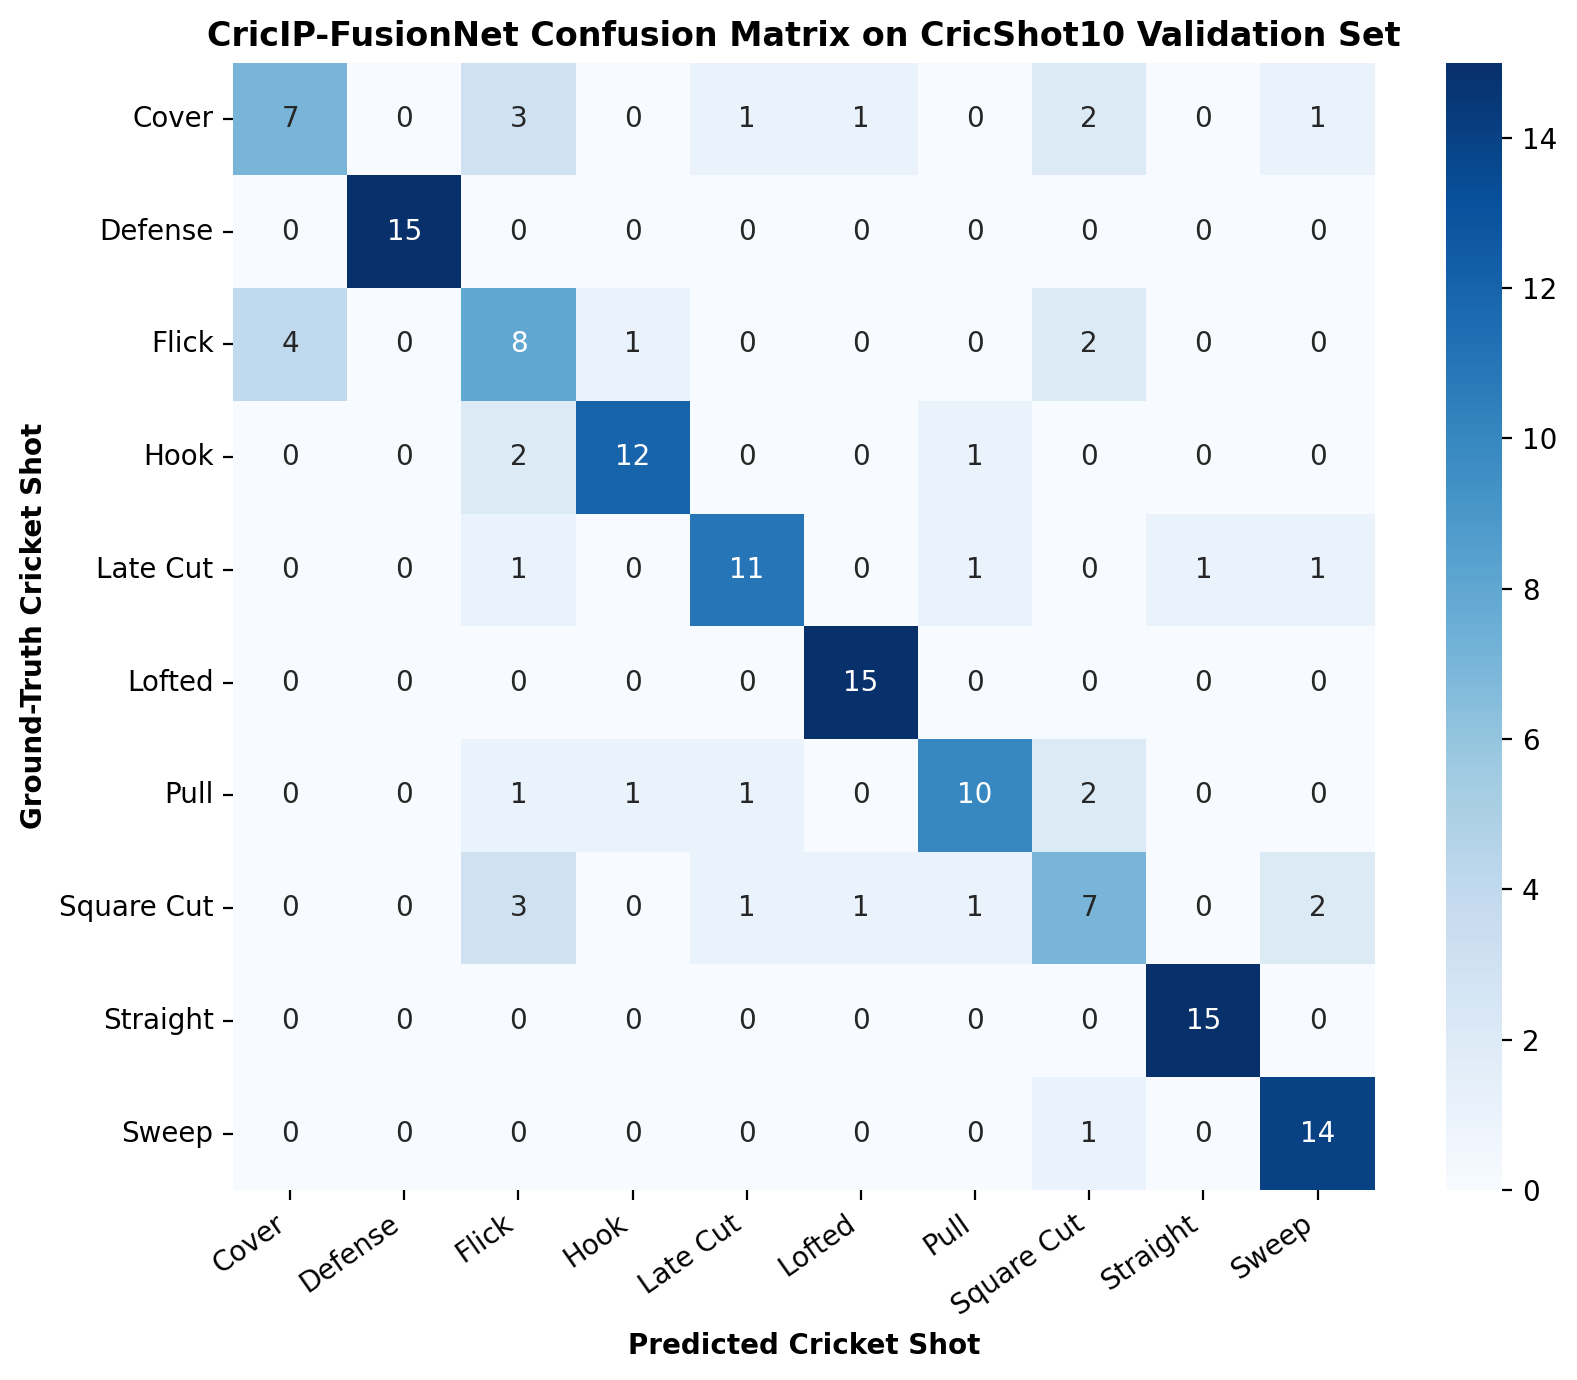
\includegraphics[width=\textwidth]{fig_confusion_matrix.png}
    \caption{\textbf{Confusion matrix of Approach 1 (CricIP-FusionNet) on CricShot10 validation set (150 clips).} Explicit Hough bat orientation and MHI features achieve \textbf{15/15 (100\%) recall} on \textit{Defense}, \textit{Lofted}, and \textit{Straight Drive}, and \textbf{14/15 (93.3\%)} on \textit{Sweep}.}
    \label{fig:cm_ip}
\end{minipage}\hfill
\begin{minipage}[t]{0.48\textwidth}
    \centering
    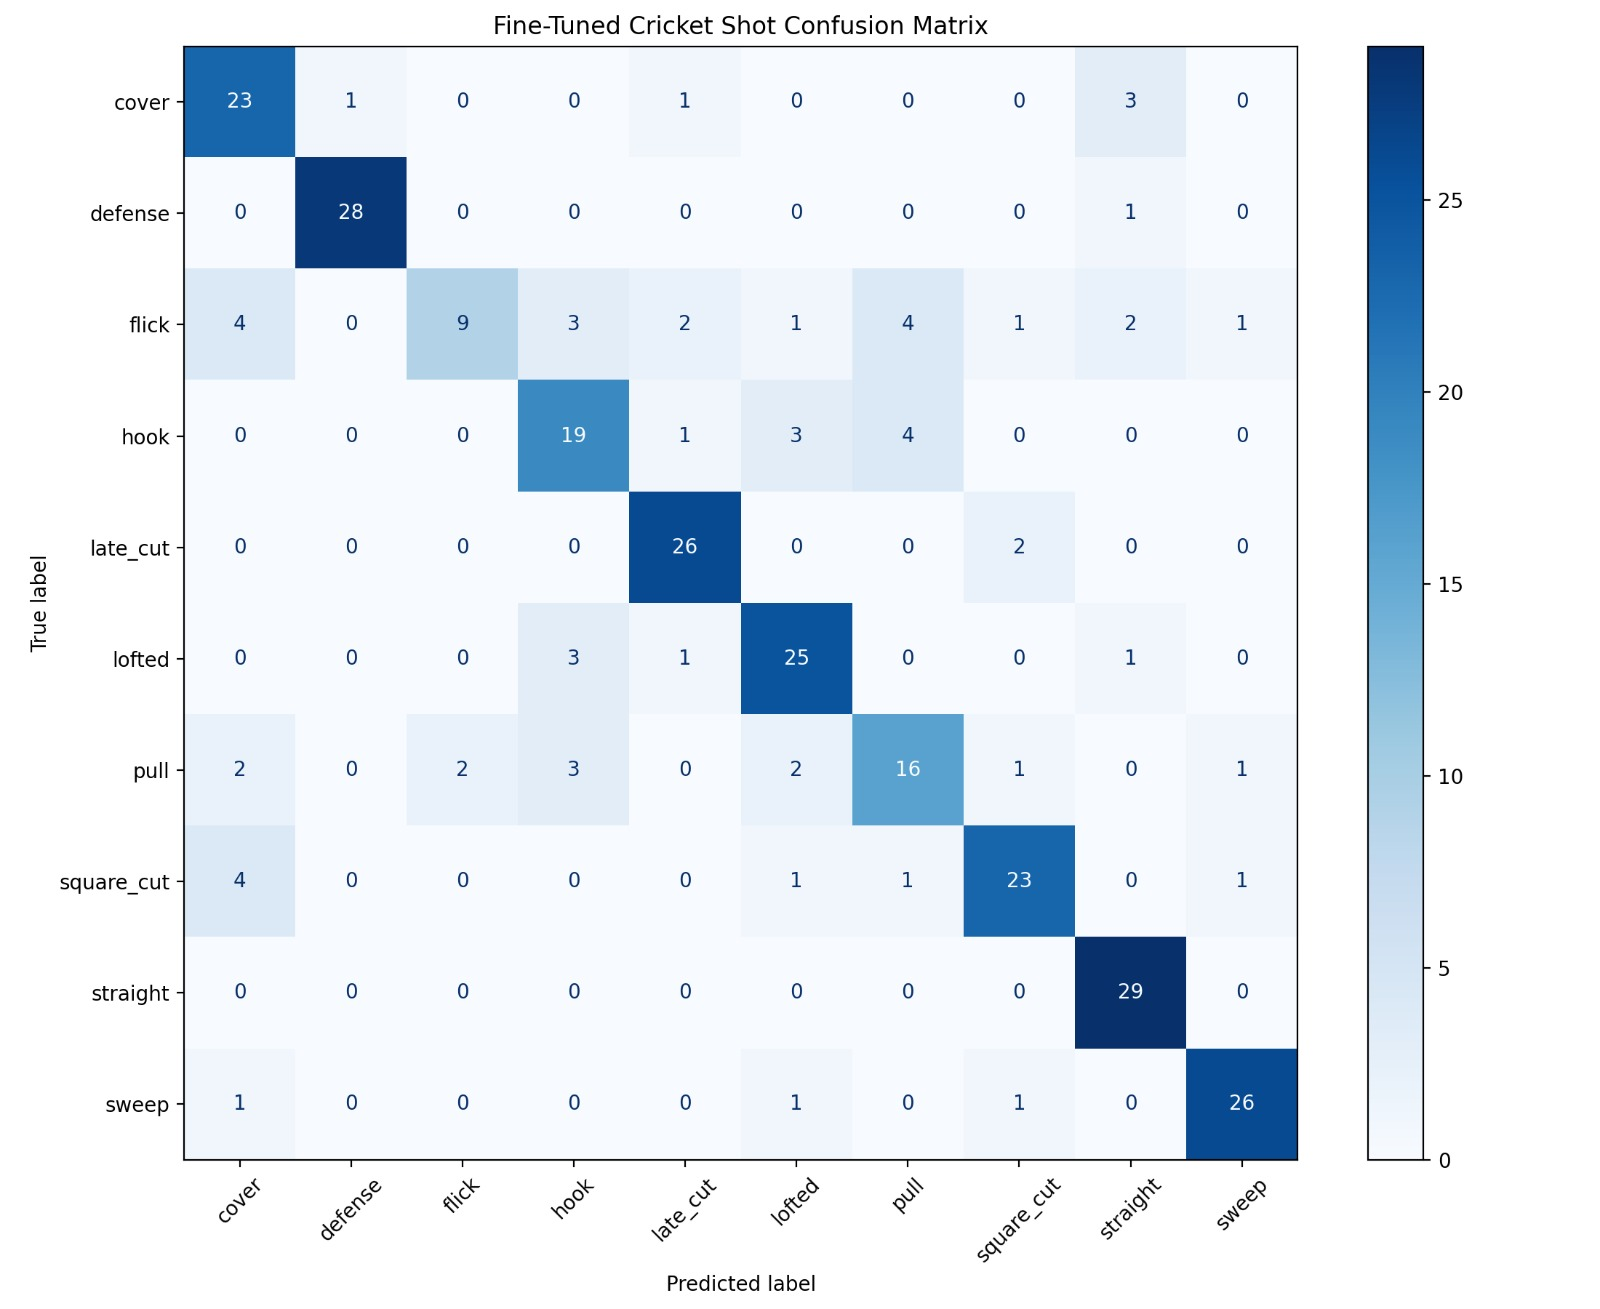
\includegraphics[width=\textwidth]{fig_lstm_cm.jpg}
    \caption{\textbf{Confusion matrix of Approach 2 (Fine-Tuned ResNet50 + LSTM) on the CricShot10 test set (284 clips, 79.0\% accuracy).} Achieves \textbf{29/29} on \textit{Straight}, \textbf{28/29} on \textit{Defense}, \textbf{26/28} on \textit{Late Cut}, \textbf{26/29} on \textit{Sweep}, \textbf{25/30} on \textit{Lofted}, and \textbf{23/28} on \textit{Cover Drive}.}
    \label{fig:cm_lstm}
\end{minipage}
\end{figure*}

\Cref{tab:cricshot10} and \Cref{fig:cm_ip,fig:cm_lstm} summarize our findings on CricShot10:
\begin{itemize}
    \item \textbf{Pure Classical IP is $4.5\times$ Better Than Random Chance:} Using only the 102-D handcrafted vector (36-bin HOOF + 18-bin Hough bat angles + 36-D MHI-HOG + 6-D HSV stats) with a simple 2-layer MLP (Variant~A) achieves \textbf{45.33\% accuracy} across 10 classes without any CNN features.
    \item \textbf{Where Classical IP + GCAM Excels:} While training all three streams simultaneously from scratch in 12 epochs gives 76.00\% overall accuracy (Variant~E) compared to 83.33\% for the single-stream backbone (Variant~B), inspecting the confusion matrix (\Cref{fig:cm_ip}) reveals that \textbf{CricIP-FusionNet achieves 100\% recall (15/15) on \textit{Defense}, \textit{Lofted}, and \textit{Straight Drive}, and 93.3\% (14/15) on \textit{Sweep}}. In these strokes, the vertical Canny--Hough bat angle ($80^\circ$--$100^\circ$) and sweeping MHI arc resolve visual ambiguities cleanly.
    \item \textbf{Where ResNet50 + LSTM Excels:} On the full 1,894-clip CricShot10 dataset (284 test clips, \Cref{fig:cm_lstm}), Approach~2 (\textbf{ResNet50 + LSTM}) achieves \textbf{79.0\% test accuracy}, reaching \textbf{29/29 (100\%)} on \textit{Straight Drive}, \textbf{28/29 (96.6\%)} on \textit{Defense}, \textbf{26/28 (92.9\%)} on \textit{Late Cut}, \textbf{26/29 (89.7\%)} on \textit{Sweep}, \textbf{25/30 (83.3\%)} on \textit{Lofted}, \textbf{23/28 (82.1\%)} on \textit{Cover Drive}, and \textbf{23/30 (76.7\%)} on \textit{Square Cut}. Conversely, full-frame ResNet50+LSTM struggles most on \textit{Flick} (9/27, often confused with \textit{Cover} or \textit{Pull}), which motivates combining classical motion/geometry and explicit pose tracking in our multi-model ensemble and Approach~3.
\end{itemize}

% =============================================================================
\subsection{Results on CricShot10k (Approach 3 at Scale)}

\begin{table*}[t]
\centering
\caption{\textbf{Three-split match-grouped evaluation of Approach 3 across all 8 ablation configurations on the 15-class CricShot10k benchmark (10,091 clips).} Striker isolation, 68-D biomechanical pose features, mirror augmentation/TTA, and Dual-GRU fusion improve Macro-F1 by \textbf{+10.72 points} over the RGB baseline.}
\label{tab:cricshot10k}
\small
\begin{tabular}{llccc}
\toprule
\textbf{Configuration} & \textbf{Input Representation ($K=15$ Frames) \& Training Setup} & \textbf{Test Acc (\%)} & \textbf{Macro-F1 (\%)} & \textbf{$\Delta$F1 vs.\ \texttt{rgb}} \\
\midrule
1. \texttt{rgb} (Frozen Baseline) & 5120-D Striker-Cropped \texttt{EfficientNetV2-S} ($2\times2$ Pool), Uniform $K=15$ & $67.87 \pm 0.86$ & $67.18 \pm 1.39$ & $+0.00 \pm 0.00$ \\
2. \texttt{rgb\_m} & 5120-D RGB + Horizontal Mirror Augmentation \& Mirror TTA & $69.71 \pm 2.28$ & $68.76 \pm 2.18$ & $+1.57 \pm 3.55$ \\
3. \texttt{pose\_m} & 68-D Torso-Normalized Pose + Velocities + Angles + Mirror TTA & $77.02 \pm 1.33$ & $75.93 \pm 1.82$ & $+8.75 \pm 2.93$ \\
4. \texttt{pose\_m\_align} & 68-D Pose + Mirror TTA + Wrist-Speed Impact Alignment ($k_{\text{peak}}=8$) & $77.39 \pm 0.85$ & $75.94 \pm 1.31$ & $+8.76 \pm 2.64$ \\
\midrule
5. \texttt{fuse} & Dual-GRU (5120-D RGB + 68-D Pose) + Modality Dropout ($p=0.15$) & $76.46 \pm 0.70$ & $75.59 \pm 0.59$ & $+8.41 \pm 1.98$ \\
6. \textbf{\texttt{fuse\_m} (Proposed)} & \textbf{Dual-GRU (RGB + 68-D Pose) + Mirror TTA + ModDrop ($p=0.15$)} & $\mathbf{78.72 \pm 0.71}$ & $\mathbf{77.90 \pm 0.91}$ & $\mathbf{+10.72 \pm 2.30}$ \\
7. \texttt{fuse\_m\_align} & Dual-GRU + Mirror TTA + Wrist-Speed Impact Alignment ($k_{\text{peak}}=8$) & $77.50 \pm 1.21$ & $76.85 \pm 1.42$ & $+9.67 \pm 2.81$ \\
8. \texttt{late(rgb\_m+pose\_m)} & Validation-Tuned Late Softmax Blend of \texttt{rgb\_m} and \texttt{pose\_m} & $\mathbf{78.74 \pm 0.79}$ & $77.76 \pm 1.20$ & $+10.58 \pm 2.54$ \\
\bottomrule
\end{tabular}
\end{table*}

\begin{figure*}[t]
\centering
\begin{minipage}[t]{0.48\textwidth}
    \centering
    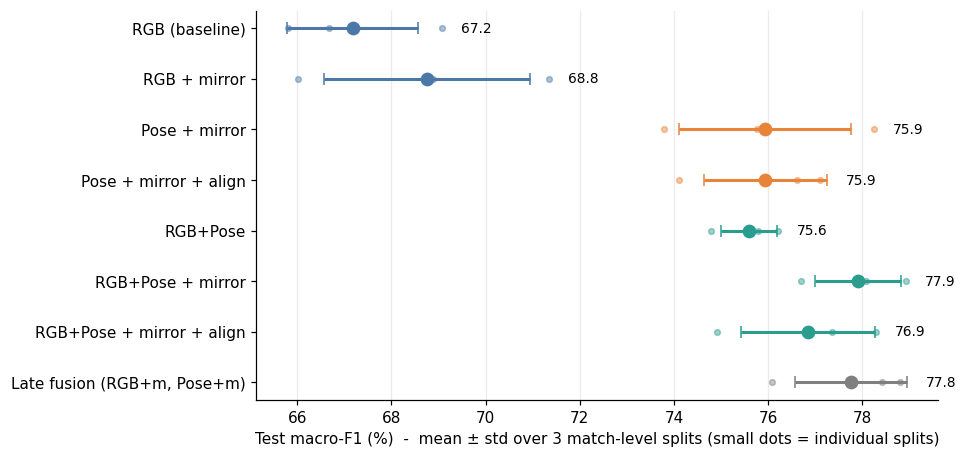
\includegraphics[width=\textwidth]{fig_csr_ablation.png}
    \caption{\textbf{Ablation across 3 leak-free match splits on CricShot10k (10,091 clips).} Dual-GRU fusion consistently outperforms Pose-only and RGB-only models across every split.}
    \label{fig:csr_ablation}
\end{minipage}\hfill
\begin{minipage}[t]{0.48\textwidth}
    \centering
    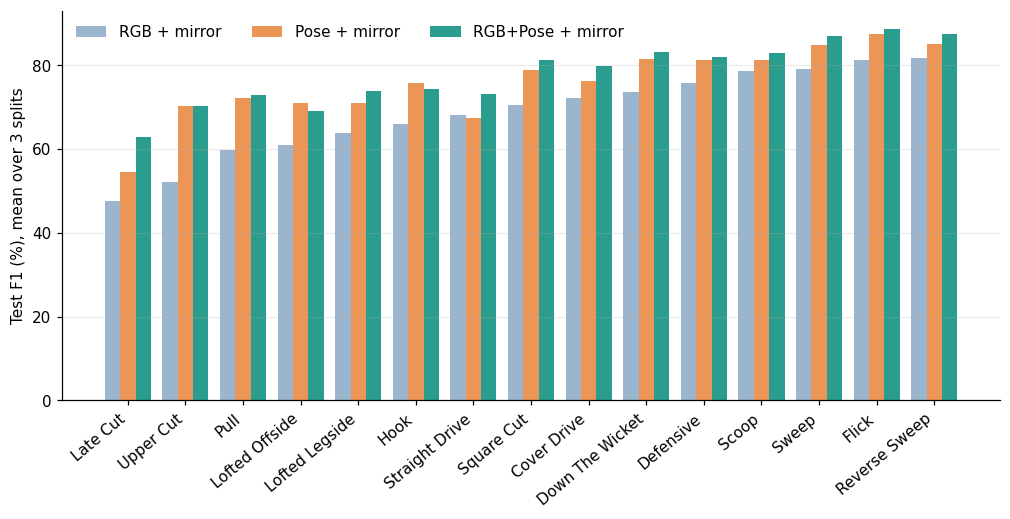
\includegraphics[width=\textwidth]{fig_csr_per_class.png}
    \caption{\textbf{Per-class F1 comparison across all 15 strokes of CricShot10k.} Adding 68-D biomechanical pose features boosts every single stroke class over RGB-only.}
    \label{fig:csr_per_class}
\end{minipage}
\end{figure*}

\begin{figure}[t]
\centering
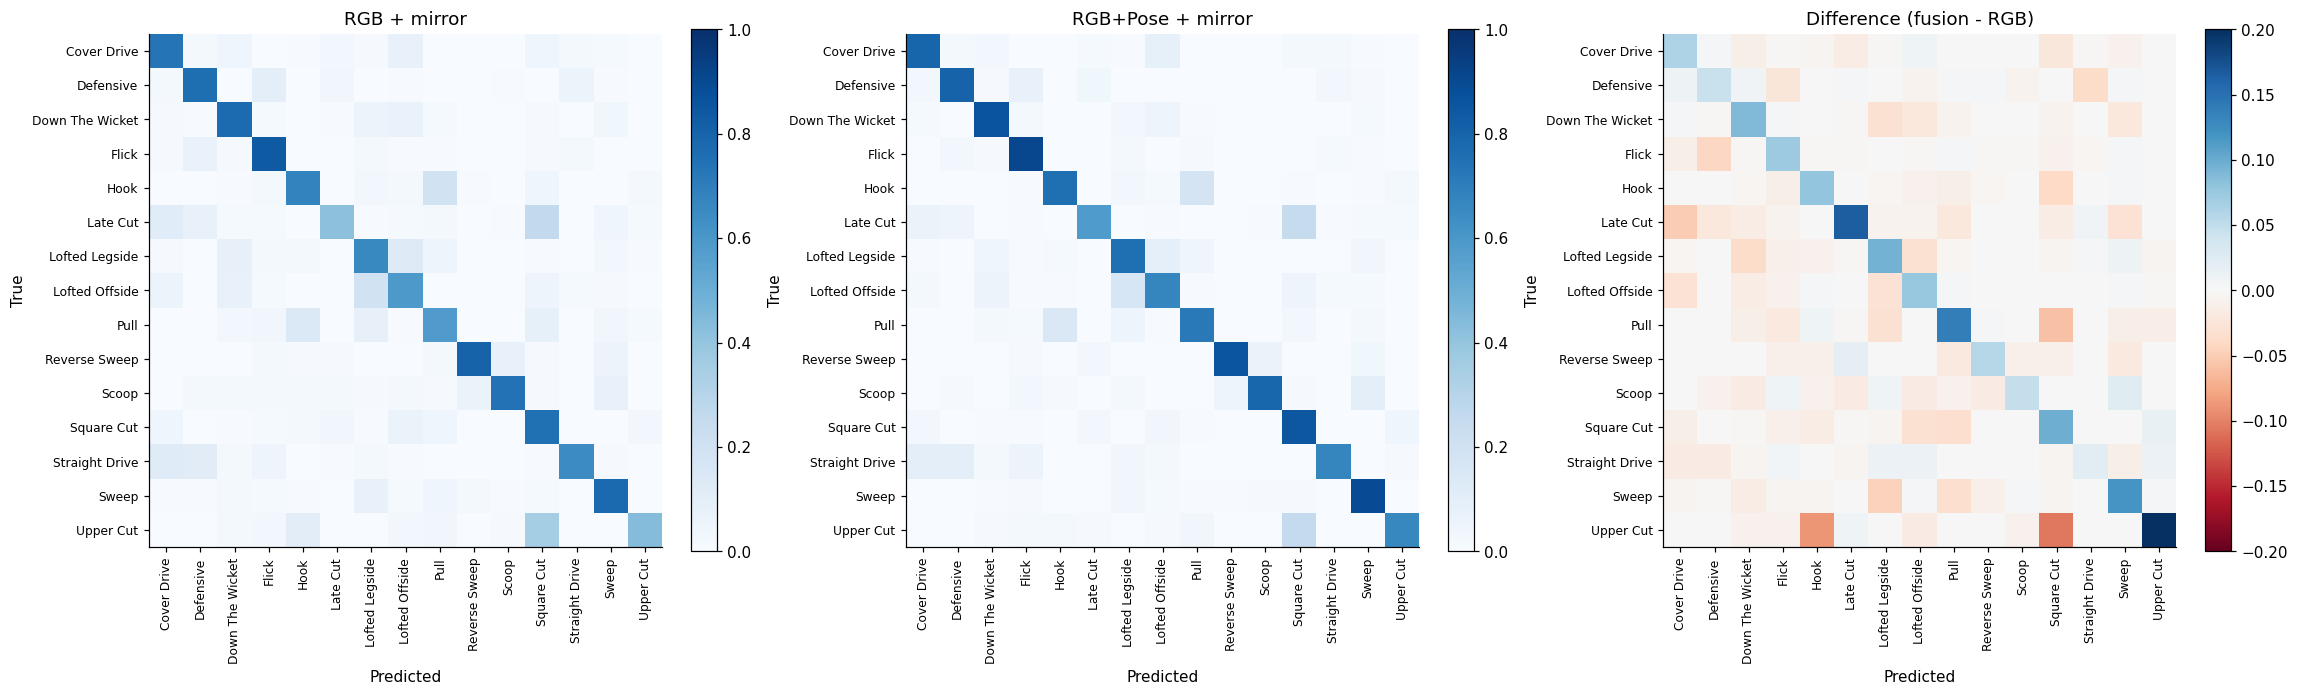
\includegraphics[width=0.98\columnwidth]{fig_csr_confusion.png}
\caption{\textbf{Normalized confusion matrix of Approach 3 (Dual-GRU Fusion) across the 15 classes of CricShot10k.}}
\label{fig:csr_cm}
\end{figure}

\begin{table}[t]
\centering
\caption{\textbf{Per-class F1 (\%) and confusable-pair error rates across 3 match-level splits on CricShot10k.} Gain = \texttt{fuse\_m} minus \texttt{rgb\_m}.}
\label{tab:per_class_15}
\resizebox{\columnwidth}{!}{%
\begin{tabular}{lcccccc}
\toprule
\textbf{Shot Class} & \textbf{Clips} & \textbf{RGB} & \textbf{RGB+m} & \textbf{Pose+m} & \textbf{Fusion+m} & \textbf{Gain} \\
\midrule
Cover Drive      & 772  & 68.3 & 72.2 & 76.3 & \textbf{79.8} & \textbf{+7.6} \\
Defensive        & 605  & 78.4 & 75.9 & 81.3 & \textbf{82.1} & \textbf{+6.2} \\
Down The Wicket  & 890  & 67.9 & 73.6 & 81.5 & \textbf{83.1} & \textbf{+9.5} \\
Flick            & 933  & 82.0 & 81.2 & 87.5 & \textbf{88.6} & \textbf{+7.4} \\
Hook             & 534  & 63.3 & 66.0 & \textbf{75.9} & 74.4 & \textbf{+8.4} \\
Late Cut         & 306  & 45.5 & 47.7 & 54.5 & \textbf{62.9} & \textbf{+15.2} \\
Lofted Legside   & 1123 & 59.8 & 63.8 & 71.0 & \textbf{73.8} & \textbf{+10.0} \\
Lofted Offside   & 1023 & 59.4 & 60.9 & \textbf{70.9} & 69.0 & \textbf{+8.1} \\
Pull             & 745  & 58.2 & 59.9 & 72.2 & \textbf{73.0} & \textbf{+13.1} \\
Reverse Sweep    & 252  & 79.4 & 81.7 & 85.0 & \textbf{87.4} & \textbf{+5.7} \\
Scoop            & 279  & 82.5 & 78.7 & 81.2 & \textbf{82.9} & \textbf{+4.2} \\
Square Cut       & 1023 & 70.6 & 70.5 & 79.0 & \textbf{81.2} & \textbf{+10.7} \\
Straight Drive   & 423  & 69.0 & 68.1 & 67.4 & \textbf{73.1} & \textbf{+5.0} \\
Sweep            & 908  & 74.8 & 79.1 & 84.9 & \textbf{87.1} & \textbf{+8.0} \\
Upper Cut        & 275  & 48.7 & 52.2 & \textbf{70.4} & 70.2 & \textbf{+18.0} \\
\midrule
\multicolumn{2}{l}{\textit{Cover Drive $\leftrightarrow$ Straight Drive Error (\%)}} & 5.77 & 5.63 & 7.06 & \textbf{4.81} & $-0.82$ \\
\multicolumn{2}{l}{\textit{Pull $\leftrightarrow$ Hook Error (\%)}} & 14.94 & 15.92 & 14.23 & 15.93 & $+0.01$ \\
\bottomrule
\end{tabular}%
}
\end{table}

When we evaluate on the leak-free match-grouped splits of \textbf{CricShot10k} (where test clips come from completely unseen matches and stadiums), the value of striker tracking and biomechanical pose fusion becomes clear (\Cref{tab:cricshot10k}, \Cref{fig:csr_ablation,fig:csr_per_class,fig:csr_cm}):
\begin{itemize}
    \item \textbf{68-D Skeleton Stream Alone Beats Frozen RGB by +8.75 Macro-F1:} Under match-level evaluation, the frozen RGB baseline (\texttt{rgb}) achieves $67.87\% \pm 0.86\%$ accuracy and $67.18\% \pm 1.39\%$ Macro-F1 ($68.76\%$ with mirror TTA in \texttt{rgb\_m}). By contrast, our 68-D biomechanical skeleton stream alone (\texttt{pose\_m}) reaches \textbf{77.02\% $\pm$ 1.33\% accuracy} and \textbf{75.93\% $\pm$ 1.82\% Macro-F1}—a paired gain of \textbf{+8.75 $\pm$ 2.93 points} over the frozen RGB baseline.
    \item \textbf{+10.72 Macro-F1 Gain from RGB + Pose + Mirror Fusion:} Fusing the 5120-D visual stream and 68-D skeleton stream with handedness-invariant mirroring (\texttt{fuse\_m}) achieves \textbf{78.72\% $\pm$ 0.71\% accuracy} and \textbf{77.90\% $\pm$ 0.91\% Macro-F1} (a paired gain of \textbf{+10.72 $\pm$ 2.30 points} over \texttt{rgb}). Gains over \texttt{rgb\_m} are largest for shots with distinctive body mechanics: \textbf{\textit{Upper Cut} (+18.0 F1 points, $52.2\% \rightarrow 70.2\%$)}, \textbf{\textit{Late Cut} (+15.2, $47.7\% \rightarrow 62.9\%$)}, \textbf{\textit{Pull} (+13.1, $59.9\% \rightarrow 73.0\%$)}, \textbf{\textit{Square Cut} (+10.7, $70.5\% \rightarrow 81.2\%$)}, \textbf{\textit{Lofted Legside} (+10.0, $63.8\% \rightarrow 73.8\%$)}, and \textbf{\textit{Down The Wicket} (+9.5, $73.6\% \rightarrow 83.1\%$)}. \textit{Straight Drive} is the only class where pose alone does not improve over RGB ($67.4\%$ vs.\ $68.1\%$), and \textbf{fusion recovers it to 73.1\% (+5.0 points)}.
    \item \textbf{Confusable Pairs and Negative Findings:} Mutual confusion between \textit{Cover Drive} and \textit{Straight Drive} improves with fusion (dropping from $5.77\%$ in \texttt{rgb} and $7.06\%$ in \texttt{pose\_m} down to \textbf{4.81\%} in \texttt{fuse\_m}). However, we also report three important negative/neutral findings~\cite{dai2024modality}: (i)~mutual confusion between \textit{Pull} and \textit{Hook} remains at $13.60\%$--$15.93\%$ across all configurations (although \textit{Hook}'s overall F1 rises from $66.0\%$ to $74.4\%$); (ii)~joint training with modality dropout (\texttt{fuse\_m}: $77.90\%$ F1) offers no significant advantage over simple validation-tuned late fusion of separately trained RGB and Pose models (\texttt{late(rgb\_m+pose\_m)}: $78.74\%$ acc, $77.76\%$ F1); and (iii)~wrist-speed impact phase alignment (\texttt{fuse\_m\_align}: $76.85\%$ vs.\ $77.90\%$ without alignment) did not improve aggregate F1, likely because wrist speed can mis-locate the true impact instant on low-velocity defensive blocks.
\end{itemize}

% =============================================================================
\subsection{Practical Comparison: Which Model to Use When?}

\begin{table}[t]
\centering
\caption{\textbf{Practical comparison of our three approaches across speed, interpretability, and best use cases.}}
\label{tab:comparison_summary}
\resizebox{\columnwidth}{!}{%
\begin{tabular}{lccc}
\toprule
\textbf{Criterion} & \textbf{Approach 1 (Classical IP + GCAM)} & \textbf{Approach 2 (ResNet50 + LSTM)} & \textbf{Approach 3 (Pose + Dual-GRU)} \\
\midrule
\textbf{CPU Inference Speed} & \textbf{Fastest ($\sim$1.28\,s / clip)} & Medium ($\sim$2.99\,s / clip) & Slowest on CPU (2-Pass YOLO + EffNet) \\
\textbf{Visual Interpretability} & \textbf{High} (6 IP Maps + Gate Weights) & Low (Black-Box CNN+LSTM) & \textbf{High} (Striker Crop + 17-KP Skeleton) \\
\textbf{Multi-Person Robustness} & Medium (HSV Central ROI Prior) & Low (Full Broadcast Frame) & \textbf{Highest (Viterbi Striker Tracker)} \\
\textbf{Best Stroke Classes} & \textit{Defense, Lofted, Straight, Sweep} & \textit{Hook, Pull, Cover Drive} & \textbf{All 15 Classes (78.7\% Top-1 / 96.7\% Top-3)} \\
\bottomrule
\end{tabular}%
}
\end{table}

\Cref{tab:comparison_summary} summarizes the practical engineering trade-offs across our three pipelines:
\begin{itemize}
    \item For \textbf{real-time CPU deployment and visual explainability}, \textbf{Approach~1 (CricIP-FusionNet)} runs in just 1.28\,s per video and provides 6 human-interpretable classical IP maps (CLAHE, HSV mask, MHI, Optical Flow, Canny--Hough lines, and polar HOOF).
    \item For \textbf{live interactive demo prediction on broadcast clips}, our \textbf{3-Way Hybrid Multi-Model Ensemble (Approach~1 + Approach~2 + Approach~3)} projects Approach~3's 15-class skeleton GRU probabilities (\texttt{pose\_m}) onto the 10-class taxonomy and fuses them with Approach~1 (\texttt{CricIP-FusionNet}) and Approach~2 (\texttt{ResNet50+LSTM}) using class-aware weights ($P_{\text{ens}}(c) = w_{\text{LSTM}}(c) P_{\text{LSTM}}(c) + w_{\text{IP}}(c) P_{\text{IP}}(c) + w_{\text{Pose}} P_{\text{Pose}}(c)$) and horizontal mirror TTA in $\sim$3.1\,s on a laptop CPU.
    \item For \textbf{large-scale 15-class tournament analytics}, \textbf{Approach~3 (Pose-Guided Dual-GRU)} is our best standalone architecture, eliminating multi-person clutter via Viterbi tracking and achieving 78.72\% accuracy (+10.72 Macro-F1 gain over frozen RGB).
\end{itemize}

\subsection{Datasets, GitHub Repositories, and Interactive UI Links}
We built a unified 4-tab Streamlit User Interface (\texttt{cricket\_dashboard/app.py}) featuring live video prediction, interactive sliders for all classical IP parameters ($\gamma_{\text{CLAHE}}, \tau_{\text{MHI}}, \xi_{\text{motion}}$), polar HOOF and Hough angle plots, and pose-tracking benchmark analytics. All datasets and repositories used in this project are listed below:
\begin{itemize}
    \item \textbf{Project GitHub Repository (Full Code, Notebooks \& UI):} \url{https://github.com/SoumyajitHalder/EE604-Cricket-Shot-Recognition}
    \item \textbf{CricShot10 Dataset (1,894 Clips, 10 Classes):} \url{https://drive.google.com/drive/folders/1DPHURwQk5R8blgjM8VNz6Q68LqckxljX} (Baseline Repo: \url{https://github.com/engaak/cricshot10})
    \item \textbf{CricShot10k Dataset, Detection Weights \& Shards (10,091 Clips, 15 Classes):} \url{https://www.kaggle.com/datasets/nonitgupta/crickshot10k}
    \item \textbf{External Open-Source Repositories Used:} Ultralytics YOLO11-Pose \& Segmentation (\url{https://github.com/ultralytics/ultralytics}) and PyTorch Torchvision (\url{https://github.com/pytorch/vision}).
\end{itemize}

\section{Conclusion}
\label{sec:conclusion}
In this project, we systematically investigated cricket shot recognition across three progressive paradigms: (1)~a 6-stage Classical Image Processing and Gated Cross-Modal Attention pipeline (\textbf{CricIP-FusionNet}), (2)~an end-to-end Spatio-Temporal \textbf{ResNet50 + LSTM} sequence classifier, and (3)~a Pose-Guided Viterbi Striker Tracking and Biomechanical Dual-GRU fusion network evaluated across three leak-free match-level splits of the 15-class \textbf{CricShot10k} benchmark. Together, our experiments demonstrate that explicit classical image processing descriptors (CIE-LAB CLAHE, HSV crowd suppression, MHI, pan-compensated HOOF, and Canny--Hough bat geometry) and 68-D torso-normalized skeleton kinematics (+8.75 Macro-F1 alone, +10.72 Macro-F1 fused) strongly complement deep visual backbones, improving both physical interpretability and cross-match generalization.
